\documentclass{csnotes}
\usepackage{xcolor}
\usepackage[italian]{babel}
\usepackage{geometry}
\usepackage{graphicx}

\geometry{
    top=2cm,
    bottom=2cm,
    left=2cm,
    right=2cm
}
% Document meta
\title{Generative AI}
\author{Giuliano Savino}
\date{\today}

% Title page info
\university{Università Degli Studi Di Napoli Federico II}
\department{Dipartimento Di Ingegneria Elettrica \\ e Delle Tecnologie Dell'Informazione}
\course{Corso Di Laurea Magistrale In Informatica}
\subject{Generative AI}
\academicyear{Academic Year 2026/2027}

\begin{document}
\thispagestyle{empty}
\begin{flushright}
    \small
    \textbf{Generative Artificial Intelligence}\\
    \textit{Scritto da : Giuliano Savino}
\end{flushright}

\vspace{-0.15cm}
\noindent
\textcolor{blue!60!black}{\rule{\textwidth}{1.2pt}}
\vfill
\begin{center}

    {\Large \textbf{Generative Artificial Intelligence}}\\[0.2cm]
        
    {\large \textit{Scritto da : Giuliano Savino}}

\end{center}

\vfill

\tableofcontents
\newpage
\chapter{Introduzione}
\section{Differenza Fra Artificial Intelligence e Generative Artificial Intelligence}
La prima domanda, che ci sorge in mente quando leggiamo il nome del corso è:
\begin{center}
    \textbf{Qual è la differenza fra "Artificial Intelligence" (AI) e "Generative Artificial Intelligence" (GAI)}
\end{center}
Cerco di spiegarmi nel modo piu chiaro possibile:
\begin{itemize}
    \item \textbf{AI} : L'AI analizza dati esistenti attraverso compiti supervisionati (classificazione, regressione), 
    non supervisionati (clustering, riduzione di dimensionalità) o self-supervised 
    (es. modellazione del linguaggio), a seconda dell'approccio.
    \begin{example}{Esempio di utilizzo di AI}
        Per esempio immagina di avere tante foto di animali,l'AI analizza le immagini e classifica ciascuna immagine, quindi l'output è legato
        ai dati che abbiamo fornito
    \end{example}
    \begin{observation}{Dati supervisionati,non supervisionati e self-supervised}
        \begin{itemize}
            \item \textbf{Dati Supervisionati (Supervised learning)} : Ho un input + la risposta corretta (label)
            \item \textbf{Dati non Supervisionati (Unsupervised learning)} : Ho solamente gli input, senza una risposta corretta.
            \item \textbf{Supervisione creata dai dati (Self-supervised learning)} : Anche qui non ho label fornite da esseri umani, 
            ma costruisci automaticamente un compito supervisionato usando i dati stessi. \textbf{Cioè nascondo una parte di Informazione
            e chiedo al modello di prevederla}
            Per esempio prendiamo una frase:
            \begin{center}
                Il gatto mangia il pesce
            \end{center}
            Nascondiamo una parola
            \begin{center}
                Il gatto mangia [MASK]
            \end{center}
            e chiediamo al modello
            \begin{center}
                Qual è la parola mancante?
            \end{center}
            il target è : "pesce".

            \textbf{La cosa importante è che "pesce" non era una label fornita dall'esterno, ma stava nei dati originali e costruisco quindi un compito
            supervisionato usando i dati stessi}
        \end{itemize}
    \end{observation}
    \newpage
    \item \textbf{GAI} : Categoria di AI che genera \textbf{nuovi contenuti}, questo include
    \begin{itemize}
        \item \textbf{Generare testo}
        \item \textbf{Generare immagini}
        \item \textbf{Generare video}
        \item \dots
    \end{itemize}
    Il modello ha imparato pattern dai dati di addestramento e li usa per produrre nuovi output.
\end{itemize}
\section{Come funziona Generative AI (In generale)}
L'AI generativa è tipicamente basata sul deep learning, specialmente parliamo di modelli allenati su grandi dataset, usando neural network architectures
\begin{itemize}
    \item Transformers (GPT,BERT,\dots)
    \item GANs (Generative Adversarial Network) - popolari per le immagini
    \item VAEs (Variational Autoencoders)
\end{itemize}
\begin{figure}[h]
    \centering
    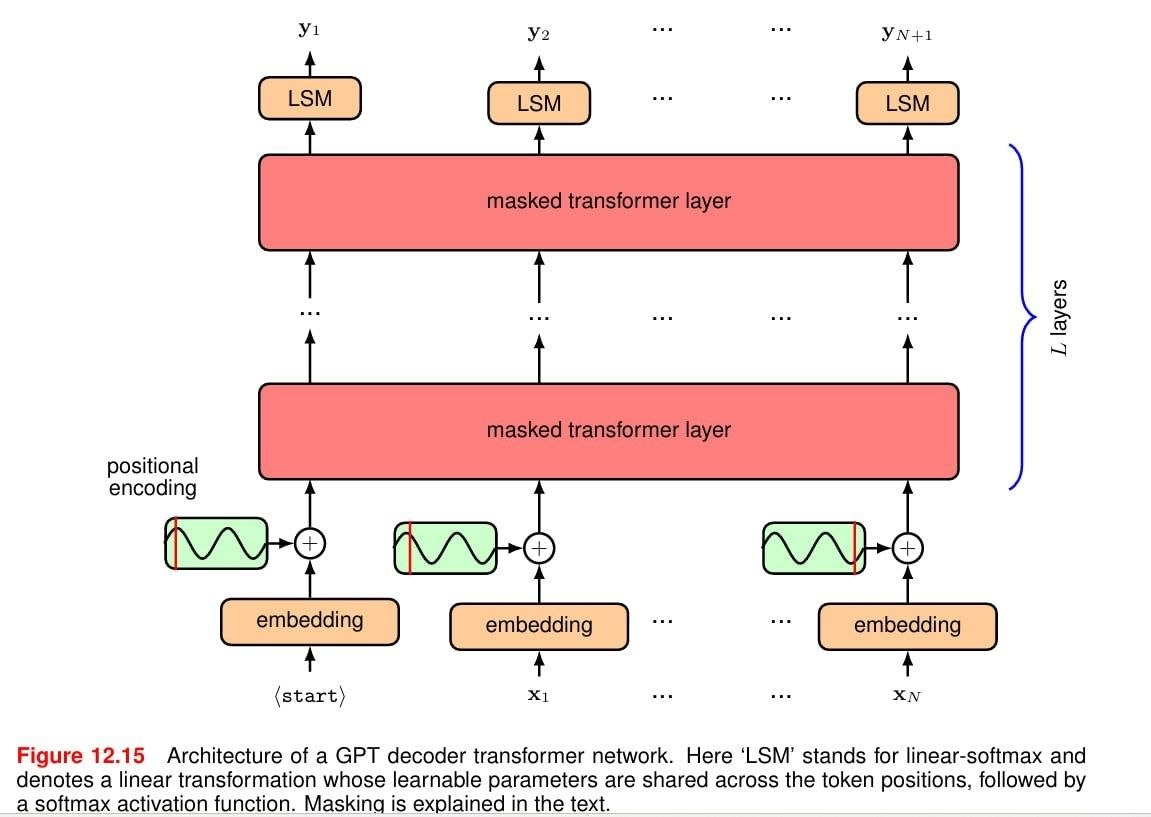
\includegraphics[width=0.8\textwidth]{_files/_images/GPT.png}
    \caption{Archittetura di GPT}
    \label{fig:GPT}
\end{figure}
Quindi in sostanza l'IA generativa,genera nuovi contenuti, come testo,immagini e audio, questo lo fa tramite modelli allenati su grandi dataset, modelli del tipo reti neurali.
Un esempio di modello che genera testo è \textbf{Generative Language Models}
\newpage
\section{Generative AI : Applicazioni e Limitazioni}
L'AI generativa trova applicazioni in:
\begin{itemize}
    \item \textbf{Creative Work}
    \item \textbf{Content Generation}
    \item \textbf{Software Development}
    \item \textbf{Education and tutoring}
    \item \textbf{Ricerche Mediche}
    \item \textbf{Generazione di testo}
\end{itemize}
ma ci sono da considerare anche i limiti che questa ha ora:
\begin{itemize}
    \item \textbf{Allucinazioni} : Le allucinazioni dell'AI sono casi in cui un modello di intelligenza artificiale genera informazioni 
    false o non supportate dai dati, presentandole però in modo plausibile e sicuro.
    Un'allucinazione non significa necessariamente che l'AI "sa che è falso e mente", la differenza è:
    \begin{itemize}
        \item \textbf{Menzogna} : Si conosce la verità,ma dico deliberatamente qualcosa di falso
        \item \textbf{Allucinazione} : L'IA genera una risposta pI Language Models sono un'applicazione della Generative AI nel dominio del testo, ovvero modelli specializzati nella generazione di linguaggio naturalelausibile,ma quella è falsa.
    \end{itemize}
    \item \textbf{DeepFakes} : l'AI genera/manipola immagini, video o audio per rappresentare una persona o un evento in modo falso.
\end{itemize}
\chapter{Language Models}
In questo capitolo ci dedicheremo ai \textbf{Language Models}.
I \textbf{Language Models} un'applicazione della \textbf{Generative AI} nel dominio del testo, quindi \textbf{modelli} specializzati nella creazione di testi.
\section{Cos'è un Language Models ?}
La classica definizione di un \textbf{Language Models}, è una \textbf{distribuzione di probabilità su una sequenza di tokens}.
Supponi noi abbiamo un vocabolario $\mathcal{V}$, di un insieme di token.
A \textbf{language model} $p$ assegna a \textbf{ciascuna} delle sequenze di token del vocabolario $x_1,\dots,x_L \in \mathcal{V}$ una probabilità (un numero fra 0 e 1)
\begin{equation}
    p(x_1,\dots,x_L)
\end{equation} 
La probabilità ci dice, intuitivamente, quanto è "buona" una sequenza di token.
Per esempio se il vocabolario è $\mathcal{V}$ = \{ate,ball,cheese,mouse,the\}, il language model assegna:
\begin{itemize}
    \item $p(the,mouse,ate,the,cheese)=0.02$
    \item $p(the,cheese,ate,the,mouse)=0.01$
    \item $p(mouse,the,the,cheese,ate)=0.0001.$
    \item \dots
\end{itemize}
In questo caso L = |$\mathcal{V}$|, ed essendo una distribuzione di probabilità:
\begin{equation}
    \sum_{x_1,\dots,x_L}p(x_1,\dots,x_L) = 1
\end{equation}


\textbf{Matematicamente quindi è un oggetto semplice e bello}, ma la semplicità è \textbf{ingannevole} : l'abilità di assegnare probabilità (meaningful) a tutte le sequenze
richiede straordinaria (ma implicita) conoscenze linguistiche e word knowledge.


Per esempio, il modello linguistico dovrebbe assegnare a «mouse the the cheese ate» una probabilità molto bassa in modo implicito
perché è grammaticalmente scorretto (conoscenza sintattica). Il modello linguistico dovrebbe assegnare a «the mouse ate the cheese» 
una probabilità più alta rispetto a «the cheese ate the mouse» in modo implicito a causa della conoscenza del mondo: entrambe le frasi 
sono identiche dal punto di vista sintattico, ma differiscono per plausibilità semantica.
\paragraph{Generation}: Come abbiamo definito, un language model $p$, prende una sequenza e ritorna una probabilità per valutarne la bontà.
Noi possiamo anche generare una sequenza dato un language model $p$.
Il modo piu teorico possibile di fare questo è andare a campionare una sequenza $x_{1:L}$ dal language model $p$, che ha probabilità $p(x_{1:L})$ (dato che ha una distribuzione di probabilità in questo modello teorico matematico posso farlo), questo si denota cosi:
\begin{equation}
    x_{1:L} \sim p
\end{equation}
Cioè l'equazione sopra significa: \textbf{estrai una sequenza di lunghezza $L$ secondo la distribuzione $p$}.
Nel modo "più puro" (teorico), ogni frase ha una probabilità di essere generata esattamente pari al suo valore $p(x_{1:L})$.
\paragraph{Perchè questa cosa è infattibile}:
Per \textbf{efficienza computazionale} \textbf{calcolare} (si perchè bisogna calcolare tutte le sequenze ovviamente) e campionare direttamente su tutte le possibili sequenze di lunghezza $L$, sarebbe
computazionalmente insostenibile, (il numero di combinazioni cresce esponenzialmente con la lunghezza $L$). Nella pratica si genera 
token per token (in modo autoregressivo).
\newpage
\section{Autoregressive language models}
Nei modelli auto-regressivi, la chain rule, ci aiuta questo perchè come abbiamo detto, il nostro problema di prima è computazionalmente intrattabile,
questo perchè se io volessi calcolare la distribuzione di probabilità congiunta $p(x_{1:L})$ senza usare la chain rule, saresti vincolato dall'assioma fondamentale della probabilità, ovvero che la somma di tutte le probabilità su tutti gli eventi possibili dello spazio campionario deve valere $1$:
cioè:
\begin{equation}
    \sum_{x_{1:L} \in V^L} p(x_{1:L}) = 1
\end{equation}
Quindi dovrei computare per ogni possibile sequenza del vocabolario fissata una lunghezza la probabilità ed è \textbf{intrattabile}.

La chain rule ci facilità il lavoro perchè io posso trovare un modo per descrivere la probabilità congiunto in un altro modo.

Un modo comune per scrivere la distribuzione congiunta $p(x_{1:L})$ di una sequenza $x_{1:L}$ consiste nell'utilizzare la \textbf{regola della catena della probabilità} (\textit{chain rule of probability}):

\[
p(x_{1:L}) = p(x_1) p(x_2 \mid x_1) p(x_3 \mid x_1, x_2) \cdots p(x_L \mid x_{1:L-1}) = \prod_{i=1}^{L} p(x_i \mid x_{1:i-1})
\]

Essendo una distribuzione di probabilità deve valere
\begin{equation}
    \sum_{(x_1,\dots,x_L \in V^L)}p(x_1,\dots,x_L) = 1 = \sum_{x_1 \in V} \sum_{x_2 \in V} \dots \prod_{i=1}^{L}p(x_i | x_{1:i-1})
\end{equation}
Ora c'è da dimostrare che 
\begin{equation}
    \sum_{x_1 \in V} \sum_{x_2 \in V} \dots \prod_{i=1}^{L}p(x_i | x_{1:i-1}) = 1
\end{equation}
Ma semplicemente posso dire che essendo ogni probabilità condizionata una distribuzione di probabilità, ad esempio fissato $x_1$:
\begin{equation}
    \sum_{x_2 \in V}p(x_2 | x_1) = 1
\end{equation}
\textbf{Portando dentro ogni sommatoria e applicando (2.7) si ha = 1}.

Passo da dover gestire uno spazio di dimensione $\vert{}V\vert{}^L$ (esponenziale) a dover fare solo $L$ passaggi, ciascuno su uno spazio di dimensione $\vert{}V\vert{}$ (lineare),
\textbf{perchè ad ogni passo, dovrò calcolarmi la distribuzione su tutti i token del vocabolario (dato i token precedenti) ed assegnare ad ogni token del vocabolario una probabilità, questo viene fatto per tutti i token della sequenza.}

Supponendo ad esempio il vocabolario di 3 token si ha dato $x_1$ = "gatto":
\begin{itemize}
    \item $p("mangia" | "gatto") = 0.8$
    \item $p("topo" | "gatto") = 0.15$
    \item $p("gatto" | "gatto") = 0.05$
\end{itemize}

e indichiamo in modo formale, ma con un piccolo abuso di notazione (perchè p indica la probabilità di un token specifico) il campionamento di $x_i$ dalla distribuzione di probabilità condizionata è:
\begin{equation}
    x_i \sim p(x_i \mid x_{1:i-1})
\end{equation}

\newpage
Un \textbf{modello di linguaggio autoregressivo} è un modello in cui ciascuna distribuzione condizionata $p(x_i \mid x_{1:i-1})$ può essere calcolata in modo efficiente (ad esempio, utilizzando una rete neurale feedforward).
\end{document}